La interpolaci\'on polinomial de Newton consiste en utilizar la base de polinomios de Newton, dada por: $\{1, x-x_0, (x-x_0)(x-x_1),\ldots,(x-x_0)(x-x_1)\cdots(x-x_{n-1})\}$, para interpolar los puntos $(x_0,y_0)$,\ldots, $(x_n,y_n)$. As\'i, el polinomio que interpola estos puntos est\'a dado por:
$$
p(x)=\alpha_0+\alpha_1(x-x_0)+\alpha_2(x-x_0)(x-x_1)+\cdots+\alpha_n(x-x_0)(x-x_1)\cdots(x-x_{n-1}),
$$
donde los coeficientes $\alpha_0,\alpha_1,\ldots,\alpha_n$ se obtienen al resolver el sistema $\boldsymbol{A\alpha}=\boldsymbol{y}$ que se obtiene al evaluar:
$$
p(x_i)=y_i,\qquad \forall\,i=0,\ldots,n.
$$
Escriba un rutero en \matlab que realice las siguientes tareas:
\begin{enumerate}
\item Construya la matriz $\boldsymbol{A}$ y el vector $\boldsymbol{y}$ mencionados anteriormente, considerando los puntos $x_i=-5,-4,\ldots,4,5$ e $y_i=1/(1+x_i^2)$.
\item Resuelva el sistema $\boldsymbol{A\alpha}=\boldsymbol{y}$ y muestre los coeficientes $a_0,\ldots, a_n$ del polinomio de interpolaci\'on de Newton. 
\item Grafique en un mismo gr\'afico la funci\'on $f(x)=1/(1+x^2)$ (l\'inea continua), el polinomio de interpolaci\'on de Newton $p(x)$ (l\'inea discontinua) y los puntos a interpolar (c\'irculos).
\end{enumerate}
>Qu\'e fen\'omeno observa en la gr\'afica? >Se puede evitar este fen\'omeno utilizando el polinomio de interpolaci\'on de Lagrange? Justifique su respuesta. \bigskip

\respuesta{3cm}
\medskip

\textbf{Desarrollo:} El rutero est\'a dado por:

\begin{lstlisting}
x = [-5:5]';
y = 1./(1+x.^2);
n = length(x);
A = ones(n,1);
aux = x - x(1);
for i=2:n
    A = [A aux];
    aux = aux.*(x - x(i));
end				%20 PUNTOS


alpha = A\y			%5 PUNTOS
xx = [-5:0.01:5]';
yy = 1./(1+xx.^2);
nn = length(xx);
aux = ones(nn,1);
pp = zeros(nn,1);
for i=1:n;
    pp = pp + alpha(i)*aux;
    aux = aux.*(xx-x(i));
end
plot(xx,yy,'-',xx,pp,'--',x,y,'o')
legend('y=1/(1+x^2)','Int. Newton', 'Puntos')		%25 PUNTOS
\end{lstlisting}
mientras que la gr\'afica est\'a dada por:

\centerline{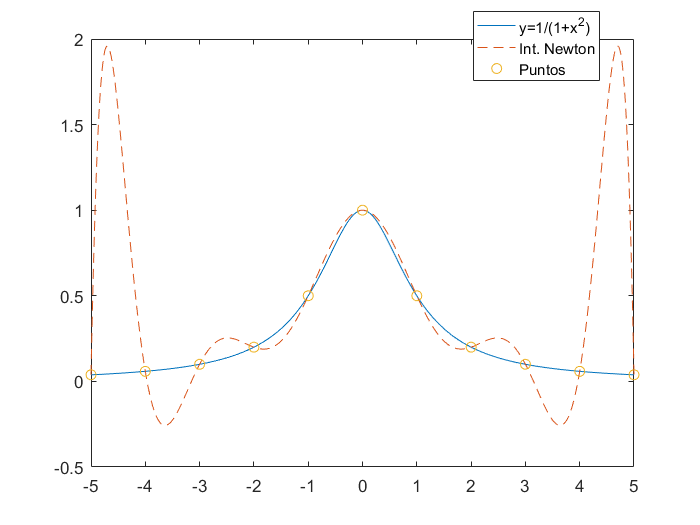
\includegraphics[width=0.6\textwidth]{inter_newton.png}}

El polinomio de interpolaci\'on de Newton presenta el fen\'omeno de Runge, el cual no puede ser evitado por la interpolaci\'on de Lagrange, debido a que el polinomio de interpolaci\'on es \'unico, independiente de la base utilizada para calcularlo (can\'onica, Lagrange o Newton).

\hfill\fbox{10 puntos}

